\documentclass[oneside,b5papar,11pt]{book}

\usepackage[protrusion=true,expansion=true]{microtype} % Better typography
\usepackage{graphicx,wrapfig} % Required for including pictures
\usepackage{mathpazo} % Use the Palatino font
\usepackage[T1]{fontenc} % Required for accented characters
\usepackage{amscd,amsmath}
\usepackage{tikz,stmaryrd}
\usepackage{latexsym,amsbsy,bbold, fullpage}
\usepackage{amssymb,amsthm,amsfonts}
\usepackage{pdfsync,yfonts}
\usepackage{tkz-graph,tikz-cd}
\usepackage[all,pdf]{xy}
\usepackage{ctex}
\usepackage{titlesec}
\usepackage{color,xcolor,tcolorbox}
\usepackage{framed}
\usepackage{hyperref,url}
\usepackage{makeidx}
\usepackage[annataritalic]{tengwarscript}%支持Tengwa字母,可以写精灵语了
\usepackage{enumitem}

\def\UrlBreaks{\do\A\do\B\do\C\do\D\do\E\do\F\do\G\do\H\do\I\do\J
\do\K\do\L\do\M\do\N\do\O\do\P\do\Q\do\R\do\S\do\T\do\U\do\V
\do\W\do\X\do\Y\do\Z\do\[\do\\\do\]\do\^\do\_\do\`\do\a\do\b
\do\c\do\d\do\e\do\f\do\g\do\h\do\i\do\j\do\k\do\l\do\m\do\n
\do\o\do\p\do\q\do\r\do\s\do\t\do\u\do\v\do\w\do\x\do\y\do\z
\do\.\do\@\do\\\do\/\do\!\do\_\do\|\do\;\do\>\do\]\do\)\do\,
\do\?\do\'\do+\do\=\do\#}%URL换行咒语

\usetikzlibrary{matrix, calc, arrows}
\usetikzlibrary{patterns,trees,snakes}

\makeindex

%%%%%%%%%%%%%%%%%%%%%%%%%%%%%%%%%%%%%%%%%%%%%%%%%%%%
%在此处调整 定义、定理、性质、引理、公理 的背景颜色%
\newcommand{\chapterbackgroundcolor}{
  \definecolor{shadecolor}{RGB}{255,227,170}
}

\newcommand*{\thmcolor}{185,181,134}
\newcommand*{\propcolor}{201,198,160}
\newcommand*{\lemmacolor}{225,225,200}
\newcommand*{\axiomcolor}{247,247,249}
\newcommand*{\definitioncolor}{173,197,165}
\newcommand*{\notationcolor}{208,222,203}
%%%%%%%%%%%%%%%%%%%%%%%%%%%%%%%%%%%%%%%%%%%%%%%%%%%%

%%%%%%%%%%%%%%%%%%%%%%%%%%%%%%%%%%%%
%%%%%这里调用了曲豆豆的独家秘籍%%%%%
%这是曲豆豆的红包

%%%%%%%%%%%%%%定理环境%%%%%%%%%%%%%%%%%%%%%%%

\newtheorem{mythm}{定理}[section]
\newtheorem{mylemma}[mythm]{引理}
\newtheorem{myprop}[mythm]{性质}
\newtheorem{myaxiom}[mythm]{公理}
\newtheorem{mydefinition}[mythm]{定义}
\newtheorem{mynotation}[mythm]{记号}
\newtheorem{example}[mythm]{例子}
\newtheorem{PreImportantExample}[mythm]{重要例子}
\newtheorem{rem}[mythm]{注记}
\newtheorem{mycor}[mythm]{推论}
\newtheorem{claim}[mythm]{断言}
\newtheorem{prob}{习题}[section]


\chapterbackgroundcolor


\newenvironment{thm}
  {\definecolor{shadecolor}{RGB}{\thmcolor}
    \begin{shaded}\begin{mythm}}
  {\end{mythm}\end{shaded}
  \chapterbackgroundcolor}

\newenvironment{lemma}
  {\definecolor{shadecolor}{RGB}{\lemmacolor}
    \begin{shaded}\begin{mylemma}}
  {\end{mylemma}\end{shaded}
  \chapterbackgroundcolor}

\newenvironment{prop}
  {\definecolor{shadecolor}{RGB}{\propcolor}
    \begin{shaded}\begin{myprop}}
  {\end{myprop}\end{shaded}
  \chapterbackgroundcolor}

\newenvironment{axiom}
  {\definecolor{shadecolor}{RGB}{\axiomcolor}
    \begin{shaded}\begin{myaxiom}}
  {\end{myaxiom}\end{shaded}
  \chapterbackgroundcolor}

\newenvironment{cor}
  {\definecolor{shadecolor}{RGB}{\lemmacolor}
    \begin{shaded}\begin{mycor}}
  {\end{mycor}\end{shaded}
  \chapterbackgroundcolor}

\newenvironment{definition}
  {\definecolor{shadecolor}{RGB}{\definitioncolor}
    \begin{shaded}\begin{mydefinition}}
  {\end{mydefinition}\end{shaded}
  \chapterbackgroundcolor}

\newenvironment{notation}
  {\definecolor{shadecolor}{RGB}{\notationcolor}
    \begin{shaded}\begin{mynotation}}
  {\end{mynotation}\end{shaded}
  \chapterbackgroundcolor}

\newenvironment{Example}
  {\definecolor{shadecolor}{RGB}{\examplecolor}
    \begin{shaded}\begin{PreImportantExample}}
  {\end{PreImportantExample}\end{shaded}
  \chapterbackgroundcolor}

%%%%%%%%%%%%%%%%%%%%%%%%%%%%%%%%%%%%%%%%%%%%%%%%%%%%%%%%%%%%
\newcommand*{\vs}{\vspace{5pt}}
\newcommand*{\vsp}{\vspace{10pt}}
\newcommand*{\vspp}{\vspace{20pt}}
\newcommand*{\kong}{$\,\,\,$}
\newcommand*{\fengexian}{
  \rule[0pt]{14.3cm}{0.01em}
\vs}
%%%%%%%%%%%%%%%%%%%%%%%%%%%%%%%%%%%%%%%%%%%%%%%%%%%%%%%%%%%%
\newcommand*{\Langle}{\left\langle}
\newcommand*{\Rangle}{\right\rangle}
%%%%%%%%%%%%%%%%%%%%%%%%%%%%%%%%%%%%%%%%%%%%%%%%%%%%%%%%%%%%
\newcommand*{\bbA}{\mathbb{A}}
\newcommand*{\bbB}{\mathbb{B}}
\newcommand*{\bbC}{\mathbb{C}}
\newcommand*{\bbD}{\mathbb{D}}
\newcommand*{\bbE}{\mathbb{E}}
\newcommand*{\bbF}{\mathbb{F}}
\newcommand*{\bbG}{\mathbb{G}}
\newcommand*{\bbH}{\mathbb{H}}
\newcommand*{\bbI}{\mathbb{I}}
\newcommand*{\bbJ}{\mathbb{J}}
\newcommand*{\bbK}{\mathbb{K}}
\newcommand*{\bbL}{\mathbb{L}}
\newcommand*{\bbM}{\mathbb{M}}
\newcommand*{\bbN}{\mathbb{N}}
\newcommand*{\bbO}{\mathbb{O}}
\newcommand*{\bbP}{\mathbb{P}}
\newcommand*{\bbQ}{\mathbb{Q}}
\newcommand*{\bbR}{\mathbb{R}}
\newcommand*{\bbS}{\mathbb{S}}
\newcommand*{\bbT}{\mathbb{T}}
\newcommand*{\bbU}{\mathbb{U}}
\newcommand*{\bbV}{\mathbb{V}}
\newcommand*{\bbW}{\mathbb{W}}
\newcommand*{\bbX}{\mathbb{X}}
\newcommand*{\bbY}{\mathbb{Y}}
\newcommand*{\bbZ}{\mathbb{Z}}

\newcommand*{\mcalA}{\mathcal{A}}
\newcommand*{\mcalB}{\mathcal{B}}
\newcommand*{\mcalC}{\mathcal{C}}
\newcommand*{\mcalD}{\mathcal{D}}
\newcommand*{\mcalE}{\mathcal{E}}
\newcommand*{\mcalF}{\mathcal{F}}
\newcommand*{\mcalG}{\mathcal{G}}
\newcommand*{\mcalH}{\mathcal{H}}
\newcommand*{\mcalI}{\mathcal{I}}
\newcommand*{\mcalJ}{\mathcal{J}}
\newcommand*{\mcalK}{\mathcal{K}}
\newcommand*{\mcalL}{\mathcal{L}}
\newcommand*{\mcalM}{\mathcal{M}}
\newcommand*{\mcalN}{\mathcal{N}}
\newcommand*{\mcalO}{\mathcal{O}}
\newcommand*{\mcalP}{\mathcal{P}}
\newcommand*{\mcalQ}{\mathcal{Q}}
\newcommand*{\mcalR}{\mathcal{R}}
\newcommand*{\mcalS}{\mathcal{S}}
\newcommand*{\mcalT}{\mathcal{T}}
\newcommand*{\mcalU}{\mathcal{U}}
\newcommand*{\mcalV}{\mathcal{V}}
\newcommand*{\mcalW}{\mathcal{W}}
\newcommand*{\mcalX}{\mathcal{X}}
\newcommand*{\mcalY}{\mathcal{Y}}
\newcommand*{\mcalZ}{\mathcal{Z}}

\newcommand*{\mfkg}{\mathfrak{g}}    %Lie algebra
\newcommand*{\mfkh}{\mathfrak{h}}
\newcommand*{\mfkm}{\mathfrak{m}}    %maximal ideal
\newcommand*{\mfkp}{\mathfrak{p}}    %prime ideal
\newcommand*{\mfkq}{\mathfrak{q}}

\newcommand*{\mfkgl}{\mathfrak{gl}}
\newcommand*{\mfksl}{\mathfrak{sl}}
\newcommand*{\mfkso}{\mathfrak{so}}
\newcommand*{\mfksp}{\mathfrak{sp}}

\newcommand*{\bfk}{\boldsymbol{k}}
\newcommand*{\bfp}{\boldsymbol{p}}
\newcommand*{\bfq}{\boldsymbol{q}}
\newcommand*{\bfu}{\boldsymbol{u}}
\newcommand*{\bfv}{\boldsymbol{v}}
\newcommand*{\bfw}{\boldsymbol{w}}
\newcommand*{\bfx}{\boldsymbol{x}}
\newcommand*{\bfy}{\boldsymbol{y}}
\newcommand*{\bfz}{\boldsymbol{z}}

\newcommand*{\Ahat}{\hat{A}}
\newcommand*{\Bhat}{\hat{B}}
\newcommand*{\Chat}{\hat{C}}
\newcommand*{\Dhat}{\hat{D}}
\newcommand*{\Ehat}{\hat{E}}
\newcommand*{\Fhat}{\hat{F}}
\newcommand*{\Ghat}{\hat{G}}
\newcommand*{\Hhat}{\hat{H}}

\newcommand*{\zbar}{\overline{z}}            %complex number
\newcommand*{\wbar}{\overline{w}}
\newcommand*{\taubar}{\overline{\tau}}

\newcommand*{\ftil}{\widetilde{f}}
\newcommand*{\gtil}{\widetilde{g}}
\newcommand*{\htil}{\widetilde{h}}
\newcommand*{\itil}{\widetilde{i}}
\newcommand*{\xtil}{\widetilde{x}}
\newcommand*{\ytil}{\widetilde{y}}
\newcommand*{\ztil}{\widetilde{z}}
\newcommand*{\wtil}{\widetilde{w}}

\newcommand*{\Omgtil}{\widetilde{\Omega}}

\newcommand*{\afa}{\alpha}
\newcommand*{\lmd}{\lambda}
\newcommand*{\Lmd}{\Lambda}
\newcommand*{\sgm}{\sigma}
\newcommand*{\Sgm}{\Sigma}
\newcommand*{\gma}{\gamma}
\newcommand*{\Gma}{\Gamma}
\newcommand*{\dta}{\delta}
\newcommand*{\Dta}{\Delta}
\newcommand*{\omg}{\omega}
\newcommand*{\Omg}{\Omega}
\newcommand*{\veps}{\varepsilon}
\newcommand*{\fai}{\varphi}
\newcommand*{\pai}{\varpi}

%%%%%%%%%%%%%%%%%%%%%%%%%%%%%%%%%%%%%%%%%%%%%%%%

\newcommand*{\ra}{\rightarrow}
\newcommand*{\inj}{\hookrightarrow}
\newcommand*{\surj}{\twoheadrightarrow}
\newcommand*{\xra}{\xrightarrow}
\newcommand*{\xla}{\xleftarrow}
\newcommand*{\llra}{\longleftrightarrow}
\newcommand*{\Llra}{\Longleftrightarrow}
\newcommand*{\rlim}{\varinjlim}                 %colimit,余极限,归纳极限,正向极限
\newcommand*{\llim}{\varprojlim}                %limit,极限,投射极限,逆向极限
\newcommand*{\suobing}{\lrcorner\,}             %张量的缩并

\newcommand*{\xybigrow}{\xymatrixrowsep{5pc}}   %交换图排版专用
\newcommand*{\xybigcol}{\xymatrixcolsep{5pc}}   %增大行、列间距
\newcommand*{\tabularbigrow}{\specialrule{0em}{4pt}{4pt}}

\newcommand*{\pz}{\text{---}}                   %破折号
\newcommand*{\yc}{\triangle}                    %余代数的乘法,co-product
\newcommand*{\p}{\partial}                      %偏微分、边缘算子partial
\newcommand*{\td}{\mathrm{d}}                   %微分算子d
\newcommand*{\pbar}{\overline{\partial}}        %Dolbeaut算子partial-bar
\newcommand*{\ten}{\otimes}                     %张量积tensor product
\newcommand*{\bigten}{\bigotimes}
\newcommand*{\op}{^{\text{op}}}
\newcommand*{\downdot}{_{\bullet}}              %下方黑点,用于同调代数中的链复形
\newcommand*{\ddowndot}{_{\bullet\bullet}}
\newcommand*{\updot}{^{\bullet}}
\newcommand*{\wedgeform}{\bigwedge\nolimits^}
\newcommand*{\ssubset}{\subset\!\subset}        %紧包含
\newcommand*{\vkong}{\varnothing}               %空集

%%%%%%%%%%%%%%%%%%%%%%%%%%%%%%%%%%%%%%%%%%%%%%%%
\newcommand*{\lbar}[1]{\overline{#1}}    %比较长的上横线

\newcommand*{\fps}[1]{[\![#1]\!]}        %Formal power series形式幂级数
\newcommand*{\Ls}[1]{(\!(#1)\!)}         %Laurent series     洛朗级数

\newcommand*{\Choose}[2]
  {\left[{
      #1 \atop
      #2
  }\right]}                              %快速输入小型方括号组合数

\newcommand*{\bbar}[1]
  {\overline{#1}}

\newcommand*{\pp}[1]
  {\frac{\partial   }
        {\partial #1}
  }                               %切向量场,一阶偏微分算子

\newcommand*{\pfrac}[2]
  {\frac{\partial #1}
        {\partial #2}
  }                               %一阶偏微分

\newcommand*{\ppfrac}[2]
  {\frac{\partial^2{#1}}
        {\partial{#2}^2}}          %二阶偏微分

\newcommand*{\pmfrac}[3]
  {\frac{\partial^2{#1}}
        {\partial{#2}\partial{#3}}} %二阶混合偏微分

%amsmath 宏包输入矩阵%
%matrix pmatrix bmatrix Bmatrix vmatrix Vmatrix%
%分别为无括号,小括号,中括号,大括号,竖线,双竖线%
%%%%%%%%%%%%%%%%%%%%%%%%%%%%%%%%%%%%%%%%%%%%%%%%
\DeclareMathOperator{\ad}{ad}         %adjoint
\DeclareMathOperator{\Ass}{Ass}       %Associated Prime
\DeclareMathOperator{\Aut}{Aut}       %automorphism
\DeclareMathOperator{\ch}{char}
\DeclareMathOperator{\cl}{cl}         %classical
\DeclareMathOperator{\Coder}{Coder}   %Co-derivation  并不是“码农”的意思
\DeclareMathOperator{\coker}{coker}   %co-kernel      余核
\DeclareMathOperator{\Conf}{Conf}     %Kontsevich公式当中用到了;configuration of points
\DeclareMathOperator{\Crit}{Crit}     %Critical locus
\DeclareMathOperator{\Der}{Der}       %Derivation        导子
\DeclareMathOperator{\Div}{div}       %divergence     散度
\DeclareMathOperator{\DR}{DR}         %De-Rham
\DeclareMathOperator{\End}{End}       %Endomorphism
\DeclareMathOperator{\Ext}{Ext}
\DeclareMathOperator{\ev}{ev}         %evaluation
\DeclareMathOperator{\Free}{Free}
\DeclareMathOperator{\Gal}{Gal}
\DeclareMathOperator{\HC}{HC}         %Hochschild Cyclic (co)homology
\DeclareMathOperator{\HH}{HH}         %Hochschild (co)homology
\DeclareMathOperator{\Hom}{Hom}
\DeclareMathOperator{\id}{id}         %identity
\DeclareMathOperator{\im}{Im}         %Image
\DeclareMathOperator{\Inn}{Inn}       %Inner Derivation  内导子
\DeclareMathOperator{\Inv}{Inv}
\DeclareMathOperator{\Lie}{Lie}
\DeclareMathOperator{\Mor}{Mor}       %Morphism
\DeclareMathOperator{\Obj}{Obj}
\DeclareMathOperator{\Obs}{Obs}       %Observable
\DeclareMathOperator{\per}{per}       %periodic cyclic complex
\DeclareMathOperator{\PV}{PV}         %Polyvector field
\DeclareMathOperator{\Rep}{Rep}
\DeclareMathOperator{\sgn}{sgn}
\DeclareMathOperator{\Sh}{Sh}
\DeclareMathOperator{\Span}{span}
\DeclareMathOperator{\supp}{supp}     %Support 支撑集
\DeclareMathOperator{\Sym}{Sym}       %Symmetry  对称张量积
\DeclareMathOperator{\Tor}{Tor}
\DeclareMathOperator{\Tot}{Tot}       %Total complex of a double-complex
\DeclareMathOperator{\YM}{YM}         %Yang-Mills   杨振宁-米尔斯

%%%%%%%%%%%%%%%%%%%%%%%%%%%%%%%%%%%%%%%%%%%%%%%%
%%%%%%%%%%%%以下是范畴论记号%%%%%%%%%%%%%%%%%%%%
\DeclareMathOperator{\Commu}{\mathsf{Commu}}
\DeclareMathOperator{\alg}{\mathsf{alg}}
\DeclareMathOperator{\Mod}{\mathsf{Mod}}

\newcommand*{\Modcat}[2]
    {\Mod^{#1}_{#2}}
\newcommand*{\Assalgcat}[2]
    {\mathsf{Ass}\!\text{-}\!\alg^{#1}_{#2}}
\newcommand*{\Commualgcat}[2]
    {\Commu\!\text{-}\!\alg^{#1}_{#2}} 
%%%%%%%%%%%%%%%%%%%%%%%%%%%%%%%%%%%%
%%%%%%%%%%%%%%%%%%%%%%%%%%%%%%%%%%%%

\linespread{1.2} % 调整行间距

\makeatletter
%\renewcommand\@biblabel[1]{\textbf{#1.}}
% 将参考文献的方括号 '[1]' 换成 '1.'

\renewcommand{\@listI}{\itemsep=0pt}
% Reduce the space between items in the itemize and enumerate environments and the bibliography

\renewcommand{\maketitle}{
% Customize the title - do not edit title and author name here, see the TITLE block below
\begin{center} % Right align 可以换成 “flushleft”
{\Huge\@title} % Increase the font size of the title

\vspace{50pt} % 标题与作者之间的行间距

{\Large\@author} % 作者姓名
\\\@date % Date

\vspace{20pt} % 作者与摘要之间的行间距
\end{center}
}


%\renewcommand{\abstractname}{摘要}
% Uncomment to change the name of the abstract to something else

\renewcommand{\bibname}{参考文献}
\renewcommand{\contentsname}{目录}
\renewcommand{\proofname}{证明}
\renewcommand{\indexname}{术语索引}

\titleformat{\chapter}
  {\color{blue}
    \huge\bfseries}
  {第\,\thechapter\,章}
{1em}{}

\newcommand{\mchapter}[1]{
  \begin{shaded}
    \chapter{#1}
  \end{shaded}
}



\title{\textbf{复几何}% Title
} % Subtitle

\author{\textsc{曲豆豆\,\,\,码字} % Author
\\{\textit{南七技校福利社\,\,五道口分社}}}

\date{\today\\
第01稿}

%----------------------------------------------------------------------------------------
\begin{document}

\maketitle

\vspp

\begin{figure}[ht]
\centering
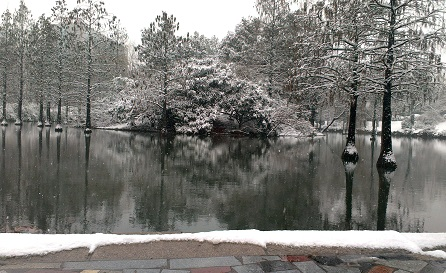
\includegraphics[width=0.7\textwidth]
  {IMAG1546.jpg}

图:中国科学技术大学西校区-也西湖雪景

拍摄于2015.1.28 - 11:30
\end{figure}

本课程参考以下教材:

1. \verb"Demailly: Complex analytic and differential geometry."

2.  \verb"Huybrechts: Complex geometry: an introduction."

3.  \verb"Morrow, Kodaira: Complex manifolds."

4. \verb"Grauert, Remmert: Coherent analytic sheaves."

5. \verb"Hormander: An introduction to complex analysis in several variables."

6. \verb"Griffiths, Harris: Principles of algebraic geometry."

\fengexian

\begin{center}
在五道口也要红专并进、理实交融呀$\sim$
\end{center}

\tableofcontents



\chapter{多复变函数}
%应该补充一些复线性空间的线性代数,单独构成一节。
\section{多元全纯函数}
首先快速回顾单复变函数的知识。
我们通常用$\Omg$来表示$\bbC$的开子集,
$z=x+iy$为$\bbC$的坐标。对于$z\in\bbC$以及实数$R>0$,我们令
$$\bbD(z,R):=\{w\in\bbC|\,|w-z|< R\}$$
为以$z$为圆心$R$为半径的开圆盘。

此外,我们有如下常用记号:
$$\left\{\begin{array}{l}
\td z:=\td x + i\td y\\
\td \bar{z} := \td x- i\td y
\end{array}\right.\quad
\left\{\begin{array}{l}
\pp{z}:=\frac{1}{2}
\left(\pp{x}-i\pp{y}\right)\\
\pp{\bar{z}} := \frac{1}{2}
\left(\pp{x}+i\pp{y}\right)
\end{array}\right.
$$
对于函数$f:\Omg\to\bbC$,
称$f$是\textbf{全纯}(holomorphic)的,
\index{holomorphic function\kong 全纯函数}
若在$\Omg$中成立
$$\pbar f:=\pfrac{f}{\bar{z}}\td\zbar=0$$
我们知道,$f$是全纯的当且仅当$f$在$\Omg$
处处能够局部地展开为收敛幂级数。

对于$\bbC$中的紧致集$K$,称函数$f:K\to\bbC$是全纯的,
如果存在$K$的开邻域$\Omg\supseteq K$,
使得$f$可延拓为$\Omg$上的全纯函数。

单复变函数论中有如下重要结果:

\begin{thm}(柯西积分公式)
设$\bbD\subseteq\bbC$为$\bbC$中的开圆盘,$f:\bbD\to\bbC$为
$\bbD$上的全纯函数,且在$\p\bbD$连续,
则对于任意$w\in\bbD$,成立
$$f(w)=\frac{1}{2\pi i}\int_{\p\bbD}\frac{f(z)}{z-w}\td z$$
\end{thm}

此定理能推导出单变量全纯函数理论的“almost everything”.
这里不再赘述。

我们开始考虑多变量全纯函数。

\begin{definition}
设$\Omg\subseteq\bbC^n$为$\bbC^n$的开子集,函数$f:\Omg\to\bbC$
称为(多变量)\textbf{全纯函数},如果满足以下条件:

(1)$f$是连续函数;

(2)对任意$1\leq j\leq n$,以及任意固定的
$z_1,...,z_{j-1};z_{j+1},...,z_n\in\bbC$,关于$z_j$的单变量函数
$$z_j\mapsto f(z_1,...,z_{j-1};z_j;z_{j+1},...,z_n)$$
是(单变量)全纯函数。
\end{definition}

事实上,如果该定义中的(2)成立,那么能推出(1)成立,
也就是说此定义中的(1)可以去掉。其证明比较复杂,我们承认之。

\begin{notation}
对于$\bbC^n$的开子集$\Omg$,我们记
$$\mcalO(\Omg):=\{f:\Omg\to\bbC|f\text{是$\Omg$上的全纯函数}\}$$
\end{notation}
容易知道$\mcalO(\Omg)$有显然的$\bbC$-代数结构。\vs

本节将说明,多变量全纯函数具有一些与单变量全纯函数类似的性质。

\begin{notation}
对于$z=(z_1,z_2,...,z_n)\in\bbC^n$以及$R=(R_1,R_2,...,R_n)\in\bbR^n$,
并且$R_j>0\,\,(\forall 1\leq j\leq n)$,则我们记
$$\bbD(z,R):=\bbD(z_1,R_1)\times\bbD(z_2,R_2)\times
\cdots\times\bbD(z_n,R_n)$$
称为以$z$为中心,$R$为半径的\textbf{多圆柱}(polydisk)。
\index{polydisk\kong 多圆柱}

对于多圆柱$\bbD(z,R)$,我们记
$$\Gamma(z,R):=\p\bbD(z_1,R_1)\times\p\bbD(z_2,R_2)\times
\cdots\times\p\bbD(z_n,R_n)$$
称为$\bbD(z,R)$的\textbf{特征边界}(distinguished boundary)。
\index{distinguished boundary\kong 特征边界}
\end{notation}
特别注意特征边界$\Gamma(z,R)$
并不等于该多圆柱的边界$\p\bbD(z,R)$.

\begin{thm}(多变量全纯函数的柯西积分公式)

设$f:\overline{\bbD(z,R)}\to\bbC$为全纯函数,
则对任意的$w\in\bbD(z,R)$,成立
$$
  f(w)=
       \frac{1}{(2\pi i)^n}\int_{\Gamma(z,R)}
         \frac{f(\xi)\td\xi_1\td\xi_2\cdots\td\xi_n}
              {(\xi_1-w_1)(\xi_2-w_2)\cdots(\xi_n-w_n)}
$$
\end{thm}
\begin{proof}
由多变量全纯函数的定义,
反复使用单变量全纯函数的柯西积分公式即可。这是容易的。
\end{proof}

与单复变函数完全类似,我们也有泰勒展开:

\begin{cor}(多元全纯函数的泰勒展开公式)

对于$f\in\mcalO(\Omg)$,其中$\Omg\subseteq\bbC^n$为开子集,则
对于任何多圆柱$\bbD(z_0,R)$,如果
$\overline{\bbD(z_0,R)}\subseteq\Omg$,则对于任意$w\in\bbD(z_0,R)$,成立
$$
  f(w)=
       \sum_{\afa\in\bbN^n}a_\afa(w-z_0)^\afa
$$
其中
$$
  a_\afa=\frac{1}{(2\pi i)^n}
           \int_{\Gamma(z_0,R)}
             \frac{f(z)}
                  {(z-z_0)^{\afa+1}}
           \td z_1\td z_2\cdots\td z_n
  =\frac{f^{(\afa)}(z_0)}{\afa!}
$$
\label{多元泰勒-cor}
\end{cor}
注意这里的$\afa$为多重指标,即$\afa=(\afa_1,...,\afa_n)$,
其中每个$\afa_i$都为非负整数。
我们记
\begin{eqnarray*}
z^{\afa}&:=&z_1^{\afa_1}z_2^{\afa_2}\cdots z_n^{\afa_n}\\
\afa!&:=&\afa_1!\afa_2!\cdots\afa_n!\\
f^{(\afa)}&:=&(\p_{z_1})^{\afa_1}(\p_{z_2})^{\afa_2}\cdots(\p_{z_n})^{\afa_n}f\\
\afa+1&:=&(\afa_1+1,\afa_2+1,...,\afa_n+1)
\end{eqnarray*}

其中$z=(z_1,...,z_n)\in\bbC^n$,$f$为$n$元全纯函数。
\begin{proof}
与单复变函数的情形完全类似,可由柯西积分公式得到。
\end{proof}

\begin{thm}(柯西不等式)对于$\bbC^n$的开子集$\Omg$,
若$f\in\mcalO(\Omg)$,多圆柱$\overline{\bbD(z_0,R)}\subseteq\Omg$,
则对任意多重指标$\afa\in\bbN^n$,成立
$$\left|f^{(\afa)}(z_0)\right|\leq
\frac{\afa!}{R^\afa}
\sup_{z\in\Gamma(z_0,R)}|f(z)|$$
\end{thm}
\begin{proof}
与单复变函数的情形完全类似。
利用多元泰勒展开(推论\ref{多元泰勒-cor})即可。
\end{proof}

\begin{cor}设$\Omg\subseteq \bbC^n$为\textbf{连通}开集,
$f\in\mcalO(\Omg)$满足$\forall 1\leq k\leq n$,
$\pfrac{f}{z_k}$在$\Omg$上恒为$0$,则$f$在$\Omg$上为常值函数。
\end{cor}

\begin{cor}(刘维尔定理)
设$f\in\mcalO(\bbC^n)$,并且满足
$$|f(z)|\leq A(1+|z|)^B$$
其中$A,B$为正实数,那么$f$必为次数不超过$B$的多项式函数。
\end{cor}

这些性质于单变量全纯函数雷同,证明也是类似的。

\begin{cor}(Montel定理)

设$\Omg$为$\bbC^n$的开子集,则$\mcalO(\Omg)$
中的任何局部一致有界的全纯函数列都存在一致收敛的子列。
\end{cor}
\begin{proof}
仍类似于单复变全纯函数的情形。使用柯西积分公式,再配合
Arzela-Ascoli定理即可。从略。
\end{proof}

现在,简单介绍一些复的微分形式。对于$\bbC^n$,记其复坐标为
$(z_1,z_2,...,z_n)$;视$\bbC^n$为$2n$维实线性空间,
$$z_k=x_k+iy_k$$
从而引入
\begin{eqnarray*}
\td z_k&=&\td x_k+i\td y_k\qquad (1,0)\text{形式}\\
\td \zbar_k&=&\td x_k-i\td y_k\qquad (0,1)\text{形式}
\end{eqnarray*}

\begin{definition}($(p,q)$-形式)

设$\Omg$为$\bbC^n$的非空开集,则形如
$$u(z)=\sum_{|I|=p\atop |J|=q}
a_{IJ}(z)\td z_I\wedge\td\zbar_J$$
的光滑张量场称为$(p,q)$-形式。
记$\Omg$上的$(p,q)$-形式之全体为$C^\infty_{p,q}(\Omg)$.
\end{definition}
这里的$I,J$为多重指标。“光滑”指的是系数函数$a_{IJ}$为$\Omg$上的光滑复值函数。
另外,显然$(0,0)$-形式即为光滑函数;
$C^\infty_{p,q}(\Omg)$具有显然的复线性空间结构,
事实上还是$C^\infty(\Omg)$-模。

\begin{notation}($\pbar$-算子)
定义算子
$$\pbar: C^\infty_{p,q}(\Omg)\to C^\infty_{p,q+1}(\Omg)$$
如下:对于$(p,q)$-形式
$$u:=\sum_{|I|=p\atop|J|=q}
a_{IJ}\td z_I\wedge\td\zbar_J$$
则
$$
  \pbar u=
  \sum_{|I|=p\atop|J|=q}
    \sum_{k=1}^n
      \pfrac{a_{IJ}}{\zbar_k}
      \td \zbar_k\wedge\td z_I\wedge\td\zbar_J
$$
\end{notation}
类似地,也有
$$\p:C_{p,q}^\infty(\Omg)\to C_{p+1,q}^\infty(\Omg)$$
它们与外微分算子$\td$满足关系
$$\td=\p+\pbar$$
由$\td^2=0$,易知
$$\p^2=0,\quad \pbar^2=0,\quad \p\pbar+\pbar\p=0$$

以下事实显然成立:
\begin{lemma}
对于区域$\Omg$上的光滑函数$f\in C^\infty(\Omg)$,
则$f$全纯当且仅当$\pbar f=0$.
\end{lemma}

\begin{rem}(Dolbeault上同调)
对于$\Omg\subseteq\bbC^n$,注意$\pbar^2=0$,
从而对任意$p\geq 0$,有上链复形$C^\infty_{p,\bullet}(\Omg)$:
$$
  \cdots\to
  C^\infty_{p,q-1}(\Omg)
  \xra{\pbar}C^\infty_{p,q}(\Omg)
  \xra{\pbar}C^\infty_{p,q+1}(\Omg)
  \to\cdots
$$
称上同调群
$$H^{p,q}(\Omg):=H^q(C^\infty_{p,\bullet}(\Omg),\pbar)$$
为区域$\Omg$的\textbf{Dolbeault上同调群}。
\index{Dolbeault cohomology}
\end{rem}
类似于外微分$\td$的de-Rham上同调群,
Dolbeault上同调群与$\Omg$的拓扑联系密切。
例如,以下定理十分重要,我们先陈述,以后再证明:

\begin{lemma}(Dolbeault-Grothendieck引理)

设$\bbD\subseteq\bbC^n$为多圆柱,则对于任意$p,q\geq 0$,
$$H^{p,q}(\bbD)=0$$
\end{lemma}

不难发现它与de Rham上同调的Poincare引理有些类似。

\section{解析延拓与Hartogs现象}
上一节介绍了多复变函数的一些“普通的”(与单变量类似)性质,
本节开始介绍多复变函数的一些独特性质。

\begin{lemma}设$f\in C^\infty_c(\bbC)$为复平面上的
紧支光滑函数,则对任意$z\in\bbC$,成立
$$
  \frac{1}{2\pi i}
  \iint_\bbC
    \frac{\p f\big/\p\taubar}
         {\tau-z}
    \td\tau\wedge\td\taubar
=f(z)$$
\end{lemma}
\begin{proof}
基本的微积分练习。考虑换元$\tau=z+re^{i\theta}$,则易知
\begin{eqnarray*}
  \td\tau\wedge\td\taubar&=&-2ir\td r\wedge\td\theta\\
  \pfrac{r}{\taubar}&=&\frac{1}{2}e^{i\theta}\\
  \pfrac{\theta}{\taubar}&=&-\frac{1}{2ir}e^{i\theta}
\end{eqnarray*}
因此有
\begin{eqnarray*}
     \frac{1}{2\pi i}
     \iint_\bbC
       \frac{\p f\big/\p\taubar}
            {\tau-z}
       \td\tau\wedge\td\taubar
&=&
     \frac{-1}{2\pi}
       \int_0^\infty\td r
         \int_0^{2\pi}
           \left(
            -\frac{1}{ir}\pfrac{f}{\theta}(z+re^{i\theta})
           \right)
           \td\theta\\
& &
    +\frac{-1}{2\pi}
     \int_0^{2\pi}\td\theta
       \int_0^\infty
       \left(
         \pfrac{f}{r}(z+re^{i\theta})
       \right)
       \td r\\
&=&
     0+\frac{-1}{2\pi}
     \int_0^{2\pi}
       -f(z)
       \td\theta\\
&=&
     f(z)
\end{eqnarray*}
证毕。
\end{proof}

\begin{lemma}(简单版本的$\pbar$-引理)

设$n\geq 2$,$\fai\in C^\infty_{0,1}(\bbC^n)$
为具有紧支集的光滑$(0,1)$-形式,
且$\pbar\fai=0$,则存在$\bbC^n$上的紧支光滑函数$g$,使得
$$\pbar g=\fai$$
\label{partial-bar引理-简单版本-lemma}
\end{lemma}

\begin{proof}
记光滑$(0,1)$-形式$\fai$为
$$\fai=\sum_{k=1}^n\fai_k(z_1,...,z_n)\td\zbar_k$$
则
\begin{eqnarray*}
     \pbar\fai
&=&
     \sum_{k,l}
       \pfrac{\fai_k}{\zbar_l}
       \td\zbar_l\wedge\td\zbar_k
 =
     \sum_{1\leq l<k\leq n}
       \left(
         \pfrac{\fai_k}{\zbar_l}
        -\pfrac{\fai_l}{\zbar_k}
       \right)
       \td\zbar_l\wedge\td\zbar_k
\end{eqnarray*}
从而由$\pbar\fai=0$可得对任意$k\neq l$,
$$\pfrac{\fai_k}{\zbar_l}=\pfrac{\fai_l}{\zbar_k}$$

考虑如下的$\bbC^n$上的函数$\psi$:对于$z=(z_1,...,z_n)\in\bbC^n$,
$$
  \psi(z)
:=
  \frac{1}{2\pi i}
  \iint_\bbC
    \frac{\fai_1(\tau;z_2,...,z_n)}
         {\tau-z_1}
    \td\tau\wedge\td\taubar
$$
由$\fai_1$的紧支性易知$\psi$为$\bbC^n$上的光滑函数。
对于$1<k\leq n$,有
\begin{eqnarray*}
     \pfrac{\psi(z)}{\zbar_k}
&=&
     \frac{1}{2\pi i}
     \iint_\bbC
       \frac{\pfrac{\fai_1}{\zbar_k}(\tau;z_2,...,z_n)}
            {\tau-z_1}
       \td\tau\wedge\td\taubar\\
&=&
     \frac{1}{2\pi i}
     \iint_\bbC
       \frac{\pfrac{\fai_k}{\taubar}(\tau;z_2,...,z_n)}
            {\tau-z_1}
       \td\tau\wedge\td\taubar\\
&=&
    \fai_k(z)
\end{eqnarray*}
上式对$k=1$显然也成立。因此$\pbar\psi=\fai$.

最后还需要证明$\psi$是紧支的。
由于$\fai$紧支,存在足够大的$R>0$,使得
$$\supp\fai\subseteq \bbD(0,R)$$
因此任意取定$z\in\bbC^n$,使得$z$的分量$z_2,z_3,...,z_n$之中
至少有一个模长大于$R$,则由$\psi$的定义式直接得到$\psi(z)=0$.
(注意:这一步严重依赖$n\geq 2$!)也就是说,存在$z\not\in\bbD(0,R)$
使得$\psi=0$在$z$的某邻域内都成立。
另一方面,由于$\pbar\psi=\fai$且$\supp\fai\subseteq\bbD(0,R)$,
从而$\psi$在$\bbD(0,\bbR)$外部全纯,因此由解析延拓唯一性,
$\psi$在$\bbD(0,R)$外部恒为零,因此$\psi$紧支。
\end{proof}

此引理在单复变$n=1$的情形\textbf{不成立}:
\begin{example}
设$\fai_1\in C_0^\infty(\bbC)$为复平面上的紧支光滑函数,并且
$$\iint_\bbC\fai_1(z)\neq 0$$
考虑$\bbC$上的$(0,1)$-形式$\fai=\fai_1(z)\td\zbar$,
则$\pbar\fai=0$是平凡的,
但\textbf{不存在}紧支光滑函数$\psi$使得$\pbar\psi=\fai$.
\end{example}

\begin{proof}
若存在紧支光滑函数$\psi$使得$\pbar\psi=\fai$,
则$\pfrac{\psi}{\zbar}=\fai_1$.于是
$$
  0\neq
  \iint_\bbC
    \fai_1(z)\td z\wedge\td\zbar
=
  \iint_\bbC
    \pfrac{\psi}{\zbar}
    \td z\wedge\td\zbar
=0
$$
产生矛盾。
\end{proof}

以下是多复变函数解析延拓的令人惊讶的性质,
它与单复变函数有本质不同:

\begin{thm}(Hartogs现象)

设$\Omg\subseteq\bbC^n$为开集$(n\geq 2)$,
$K\ssubset\Omg$且为$\bbC^n$的紧子集,
则对任意的$f\in\mcalO(\Omg\setminus K)$,
都存在解析延拓$F\in\mcalO(\Omg)$,使得
$$F|_{\Omg\setminus K}=f$$
\end{thm}

\begin{proof}
取$K$与$\Omg$直接的截断函数$\psi\in C^\infty_0(\bbC^n)$,
使得$0\leq \psi\leq 1$,
$$K\ssubset\supp\psi\ssubset\Omg$$
并且$\psi|_K\equiv 1$.
考虑$$\ftil:=(1-\psi)f$$
则$\ftil$在整个$\Omg$上都有定义。注意
$$\pbar\ftil=-(\pbar\psi)f+(1-\psi)\pbar f$$
易知$\supp\pbar\ftil\subseteq\supp\psi$.于是由
引理\ref{partial-bar引理-简单版本-lemma},存在光滑函数
$v$,使得$\supp v\subseteq\psi$,并且$\pbar v=\pbar\ftil$,
从而考虑函数
$$F:=(1-\psi)f-v$$
则$\pbar F=0$,从而$F\in\mcalO(\Omg)$.又因为易知
$$F=f\quad(\forall z\in\Omg\setminus\supp\psi)$$
从而由解析延拓唯一性,有$F_{\Omg\setminus K}=f$.
\end{proof}

关于解析延拓,再介绍如下结果:

\begin{lemma}(Hartogs figure)
\index{Hartogs figure}

对于$n>1$,正实数$0\leq r<R$,
以及$\bbC^{n-1}$的开子集$\omg'\subseteq\omg$,
其中$\omg$是连通的。记$\bbC^n$的开子集
$$
  \Omg:=
    \left(
      (\bbD(0,R)\setminus\bbD(0,r))\times\omg
    \right)
    \cup
    \left(
      \bbD(0,R)\times\omg'
    \right)
$$
其中$\bbD(0,r)$与$\bbD(0,R)$
分别为$\bbC$上的以原点为中心,$r,R$为半径的开圆盘。
则任意$f\in\mcalO(\Omg)$都可以(唯一地)解析延拓至
$$\widetilde{\Omg}:=\bbD(0,R)\times\omg$$
\end{lemma}
如此的区域$\Omg$称之为“\textbf{Hartogs figure}”。
$\Omg$的几何图像大致如下:

\begin{figure}[ht]
\centering
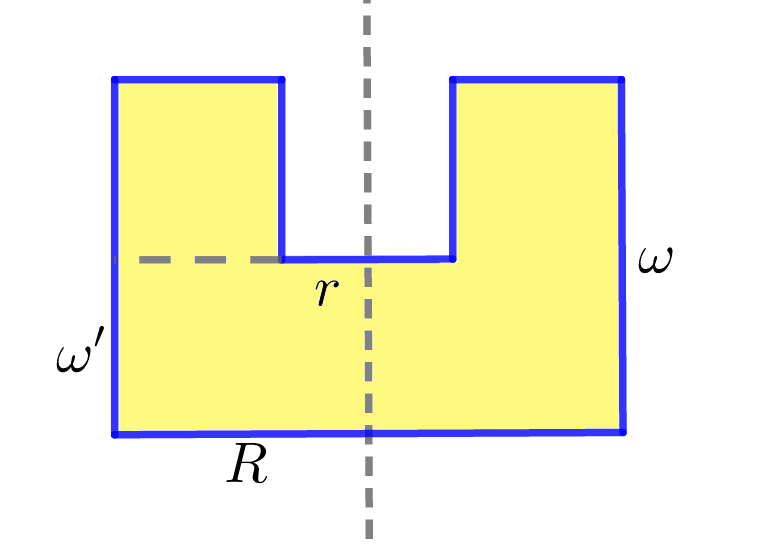
\includegraphics[width=0.4\textwidth]
  {figures/HartogsFigure.png}

图:Hartogs figure示意
\end{figure}

\begin{proof}
容易知道
$$\Omg=\big\{(z_1,\ztil)\in\bbC\times\bbC^{n-1}\big|
r<|z_1|<R,\ztil\in\omg\text{或者}
|z_1|\leq r,\ztil\in\omg'
\big\}$$
对于$f\in\mcalO(\Omg)$,定义$\Omgtil$上的函数
$$
  \ftil(z_1,\ztil):=
    \frac{1}{2\pi i}
    \int_{|w|=\rho}
      \frac{f(w,\ztil)}
           {z_1-w}
      \td w
$$
其中$\rho$为满足$\max\{r,|z_1|\}<\rho<R$的任意实数。
则易知如此定义的$\ftil$为$f$在$\Omgtil$上的解析延拓。
\end{proof}

\begin{thm}(Riemann延拓定理)

考虑$\bbC^n$中的多圆柱$\bbD(0,R)$,其中$n\geq 2$,$R\in\bbR_+^n$。
对任意$2\leq p\leq n$,令$\bbC^n$的子集
$$S:={(z_1,...,z_n)\in\bbC^n|z_1=\cdots=z_p=0}$$
则对任意$f\in\mcalO(\bbD(0,R)\setminus S)$,
$f$都可(唯一地)解析延拓至$\bbD(0,R)$.
\end{thm}

\begin{proof}
这是Hartogs figure的显然推论。记$R=(R_1,R_2,...,R_n)$,
以及$R':=(R_2,...,R_n)\in\bbR^{n-1}$.
考虑$\bbC^{n-1}$的开子集
\begin{eqnarray*}
  \omg &:=&\bbD(0,R')\\
  \omg'&:=&\omg\setminus\{z_2=\cdots=z_p=0\}
\end{eqnarray*}
则易知
$$\bbD(0,R)\setminus S=
\Big(
  \bbD(0,R_1)\setminus\{0\}\times\omg
\Big)
\cup
\Big(
  \bbD(0,R_1)\times\omg'
\Big)
$$
为Hartogs figure,从而完。
\end{proof}

\section{Weierstrass预备定理与除法定理}
(待补)









\printindex
\end{document} 